\documentclass{article}

\usepackage{fancyhdr}
\usepackage{extramarks}
\usepackage{amsmath}
\usepackage{amsthm}
\usepackage{amsfonts}
\usepackage{tikz}
\usepackage[plain]{algorithm}
\usepackage{algpseudocode}
\usepackage{amssymb}

\usetikzlibrary{automata,positioning}

%
% Basic Document Settings
%

\topmargin=-0.45in
\evensidemargin=0in
\oddsidemargin=0in
\textwidth=6.5in
\textheight=9.0in
\headsep=0.25in

\linespread{1.1}

\pagestyle{fancy}
\lhead{\hmwkAuthorName}
\chead{\hmwkClass\ (\hmwkClassInstructor\ \hmwkClassTime): \hmwkTitle}
\rhead{\firstxmark}
\lfoot{\lastxmark}
\cfoot{\thepage}

\renewcommand\headrulewidth{0.4pt}
\renewcommand\footrulewidth{0.4pt}

\setlength\parindent{0pt}

%
% Create Problem Sections
%

\newcommand{\enterProblemHeader}[1]{
    \nobreak\extramarks{}{Problem \arabic{#1} continued on next page\ldots}\nobreak{}
    \nobreak\extramarks{Problem \arabic{#1} (continued)}{Problem \arabic{#1} continued on next page\ldots}\nobreak{}
}

\newcommand{\exitProblemHeader}[1]{
    \nobreak\extramarks{Problem \arabic{#1} (continued)}{Problem \arabic{#1} continued on next page\ldots}\nobreak{}
    \stepcounter{#1}
    \nobreak\extramarks{Problem \arabic{#1}}{}\nobreak{}
}

\setcounter{secnumdepth}{0}
\newcounter{partCounter}
\newcounter{homeworkProblemCounter}
\setcounter{homeworkProblemCounter}{1}
\nobreak\extramarks{Problem \arabic{homeworkProblemCounter}}{}\nobreak{}

%
% Homework Problem Environment
%
% This environment takes an optional argument. When given, it will adjust the
% problem counter. This is useful for when the problems given for your
% assignment aren't sequential. See the last 3 problems of this template for an
% example.
%
\newenvironment{homeworkProblem}[1][-1]{
    \ifnum#1>0
        \setcounter{homeworkProblemCounter}{#1}
    \fi
    \section{Problem \arabic{homeworkProblemCounter}}
    \setcounter{partCounter}{1}
    \enterProblemHeader{homeworkProblemCounter}
}{
    \exitProblemHeader{homeworkProblemCounter}
}

%
% Homework Details
%   - Title
%   - Due date
%   - Class
%   - Section/Time
%   - Instructor
%   - Author
%

\newcommand{\hmwkTitle}{Homework\ \#3}
\newcommand{\hmwkDueDate}{November 13, 2017}
\newcommand{\hmwkClass}{Convex Optimization}
%\newcommand{\hmwkClassTime}{Section A}
\newcommand{\hmwkClassInstructor}{Professor Ying Cui}
%\newcommand{\hmwkAuthorName}{\textbf{Josh Davis} \and \textbf{Davis Josh}}
\newcommand{\hmwkAuthorName}{\textbf{Xiaoyi He}}

%
% Title Page
%

\title{
    \vspace{2in}
    \textmd{\textbf{\hmwkClass:\ \hmwkTitle}}\\
    \normalsize\vspace{0.1in}\small{Due\ on\ \hmwkDueDate\ at 11:59pm}\\
    \vspace{0.1in}\large{\textit{\hmwkClassInstructor\ \hmwkClassTime}}
    \vspace{3in}
}

\author{\hmwkAuthorName}
\date{}

%\renewcommand{\part}[1]{\textbf{\large Part \alph{partCounter}}\stepcounter{partCounter}\\}

%
% Various Helper Commands
%

% Useful for algorithms
\newcommand{\alg}[1]{\textsc{\bfseries \footnotesize #1}}

% For derivatives
\newcommand{\deriv}[1]{\frac{\mathrm{d}}{\mathrm{d}x} (#1)}

% For partial derivatives
\newcommand{\pderiv}[2]{\frac{\partial}{\partial #1} (#2)}

% Integral dx
\newcommand{\dx}{\mathrm{d}x}

% Alias for the Solution section header
\newcommand{\solution}{\textbf{\large Solution}}

% Probability commands: Expectation, Variance, Covariance, Bias
\newcommand{\E}{\mathrm{E}}
\newcommand{\Var}{\mathrm{Var}}
\newcommand{\Cov}{\mathrm{Cov}}
\newcommand{\Bias}{\mathrm{Bias}}
\newcommand{\addtag}{\refstepcounter{equation}\tag{\theequation}}

\begin{document}

\maketitle

\pagebreak
% \begin{homeworkProblem}
%     \begin{figure}[h]
%         \centering
%             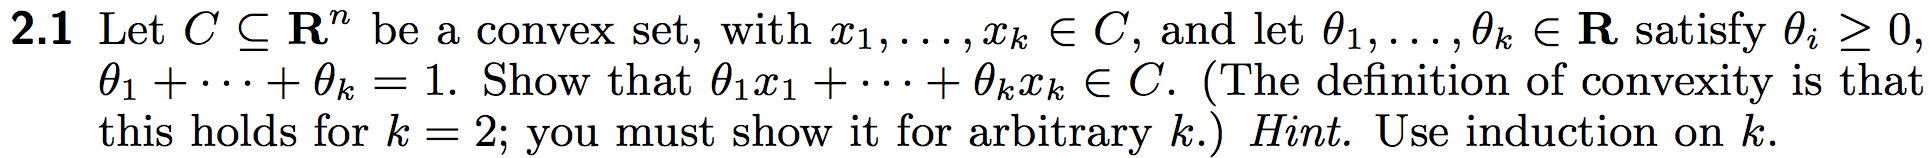
\includegraphics[width=\textwidth]{images/2-1.png}
%     \end{figure}
% \end{homeworkProblem}

\begin{homeworkProblem}
    Textbook Exercises 4.1
    \\

    \solution

    the sketch of the feasible set:
    \vskip 10\baselineskip


    (a)
    \(x^{\ast} = (2/5, 1/5)\), \(p^{\ast} = 3/5\)


    (b)
    With these constrains, \(inf\left\{f_{0}(x_{1},x_{2})\right\} = -\infty\)

    (c)
    \(X_{opt} = \{(0,x_{2})\, |\,  x_{2} \geq 1\}\), \(P^{\ast} = 0\)

    (d)
    \(x^{\ast} = (1/3, 1/3) \), \(P^{\ast} = 1/3\)

    (e)
    when the line \(x_{1} + 3x_{2} = 1 \) and the ellipsoid \(x_{2}^{2} + 9x_{2}^{2} = R^{2} \) are tangent,  the point of tangency \((x_{1}^{\ast}, x_{2}^{\ast}) \) satisfy:
    \[
       \begin{split}
        x_{1}^{\ast} + 3x_{2}^{\ast} &= 1 \\
        -x_{1}^{\ast} / 9x_{2}^{\ast} &= -1/3
        \end{split}
    \]
    Thus, \(x^{\ast} = (1/2, 1/6)\) and \(p^{\ast} = 1/2\)



\end{homeworkProblem}

\pagebreak


\begin{homeworkProblem}
    Textbook exercise 4.8 a-e
    \\

    \solution

    (a)
    If the problem is infeasible, the optimal value is \(\infty\).
    If the problem is feasible, the optimal value is \(-\infty\).

    (b)
    If the vector \(c\) is not parallel to \(a\), then the optimal value is \(-\infty\).\\
    If the vector \(c\) is equal to \(\lambda a\), the optimal value is \(-\infty\) when the \(\lambda > 0\) and the optimal value is \(\lambda b \) when \( \lambda < 0\).

    (c)
    \[p^{\ast} = \sum_{i=1}^{j} c_{i}l + \sum_{i=j+1}^{n} c_{i}u\]
     where \(c_{1},\dots, c_{j} \geq 0 \) and \(c_{j+1},\dots,c_{n} \leq 0\)

    (d)
    \[c^{T}x = \sum_{i=1}^{n} c_{i}x_{i}\]
    Let \(c_{j} = c_{min}\). Thus \(p^{\ast}  = c_{j}\) when \(x_{j}^{\ast} = 1\) and \(x_{i}^{\ast} = 0,\, i \neq j \)

    When the constraint is replaced by the inequality and \(c_{j} \leq 0\), the optimal value is achieved with \(x_{j} = 1\) and \(x_{i} = 0, \, i \neq j\). If \(c_{j} \geq 0 \) the optimal value is achieved when \(x_{i} = 0,\, i=1,\dots,n\).

    (e)
    \vskip 10\baselineskip

\end{homeworkProblem}
\pagebreak

\begin{homeworkProblem}
    Textbook exercise 4.33
    \\

    \solution

    (a) It is equivalent to:
    \[
        \begin{split}
        \text{minimize}&\ t \\
        \text{subject to}&\ \log\left(\sum_{k=1}^{K}exp(a_{ik}^{T}y + b_{ik})\right)/t \leq 1, \; i=1,2
        \end{split}
    \]

    (b) It is equivalent to:
    \[
        \begin{split}
        \text{minimize} &\ exp(t_{1}) + exp(t_{2}) \\
        \text{subject to} &\ \log\left(\sum_{k=1}^{K}exp(a_{ik}^{T}y + b_{ik})\right) \leq t_{i}, \; i = 1,2
        \end{split}
    \]

    (c)It is equivalent to:
    \[
        \begin{split}
        \text{minimize} &\ t \\
        \text{subject to} &\ \frac{\left(\log\left(\sum_{k=1}^{K}exp(a_{1k}^{T}y + b_{1k})\right)\right)/t + \log\left(\sum_{k=1}^{K}exp(a_{2k}^{T}y + b_{2k})\right)}{a^{T}y+b} \leq 1
        \end{split}
    \]

\end{homeworkProblem}
\pagebreak

\begin{homeworkProblem}
    Textbook exercise 4.40 a-c
    \\

    \solution

    (a) It is equivalent to:
    \[
        \begin{split}
        \text{minimize} &\ c^{T}x+d \\
        \text{subject to} &\ \mathbf{diag}(Gx-h) \preceq 0 \\
                        &\ Ax=b
        \end{split}
    \]

    (b)
    QP. Let \(P_{i} = W_{i}W_{i}^{T}\)
    \[
        \begin{split}
        \text{minimize} &\ t + 2q^{T}x + r \\
        \text{subject to} &\ \left[\begin{array}{cc} I & W_{T}x \\ x^{T}W & tI \end{array}\right] \succeq 0 \\
                        &\ \mathbf{diag}(Gx-h) \preceq 0 \\
                        &\ Ax = b
        \end{split}
    \]
    QCQP. Let \(P_{i} = W_{i}W_{i}^{T}\)
    \[
        \begin{split}
        \text{minimize} &\ t_{0} + 2q_{0}^{T}x + r_{0} \\
        \text{subject to} &\ \left[\begin{array}{cc} I & W_{i}^{T}x \\ x^{T}W_{i} & t_{i}I \end{array}\right] \succeq 0,\, i=0,1,\dots,m \\
                        &\ t_{i} + 2q_{i}^{T}x + r_{i} \leq 0, \, i=1,\dots,m \\
                        &\ Ax = b
        \end{split}
    \]
    SOCP.
    \[
        \begin{split}
        \text{minimize} &\ c^{T}x \\
        \text{subject to} &\ \left[\begin{array}{cc}(c_{i}^{T}x + d_{i})I & A_{i}x + b_{i} \\ (Ax_{i} + b_{i})^{T} & (c_{i}^{T} + d_{i})I \end{array}\right] \succeq 0, \, i=1,\dots,N \\
        &\ Fx=g
        \end{split}
    \]


    (c)
    \[
        \begin{split}
        \text{minimize} &\ t \\
        \text{subject to} &\ \left[ \begin{array}{cc} F(x) & Ax+b \\ (Ax+b)^{T} & t \end{array}\right] \succeq 0
        \end{split}
    \]
\end{homeworkProblem}

\pagebreak

\begin{homeworkProblem}


\end{homeworkProblem}

\end{document}
